%%% Výkresovka - textové přepisy návodů
\chapter{Výkresová dokumentace - vybrané návody}
Tato kapitola obsahuje text. přepis dvou návodů na nejběžnější operace v~sestavách.
Text je brán jako doplněk videí vypsaných v~kapitole \ref{videa-sestavy} přílohy \ref{released-videos}.

\section{Popisové pole a uživatelské vlastnosti}
Popisové pole je nedílnou součástí každého výkresu.
Udává údaje o~dané součásti, nebo sestavě, jako je označení, materiál, rozměr a podobně.
V~SolidWorks se vyplňování popisového pole řeší pomocí uživatelských vlastností, které se následně automaticky propisují na výkres.
Pro to, aby tyto vlastnosti správně fungovaly je nutné mít správně nainstalované šablony.
Jejich instalace je popsaná v~návodu \ref{instalace-sablon}.

\begin{figure}[htbp]
    \centering
    \begin{minipage}[b]{0.45\textwidth}
        \centering
        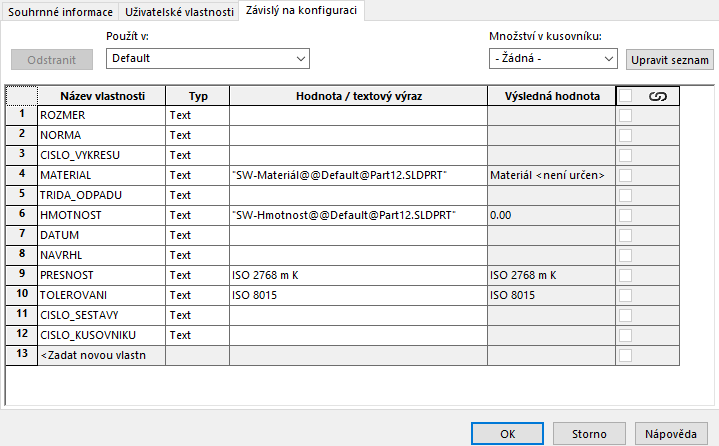
\includegraphics[width=1\textwidth]{img/030 img/vlastnosti-dilu.png}
        \caption{Tabulka vlastností souč.}
        \label{fig:realview-1}
    \end{minipage}
    \qquad
    \begin{minipage}[b]{0.45\textwidth}
        \centering
        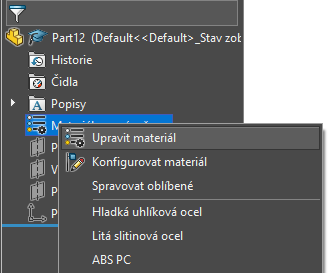
\includegraphics[width=0.7\textwidth]{img/030 img/upravit-material.png}
        \caption{Tl. pro změnu materiálu}
        \label{fig:realview-2}
    \end{minipage}
\end{figure}

Otevřeme si díl, kterému chceme upravit vlastnosti.
V~nabídce \B{Soubor} vybereme možnost \B{Vlastnosti}.
Zobrazí se nabídka vlastností dílu, ve které se musíme přepnout na kartu \B{Závislý na konfiguraci}.
Ve sloupci \B{Hodnota/textový výraz} můžeme měnit položky popisového pole.
Jakmile podle potřeby nastavíme všechny hodnoty, uložíme změny stiskem tlačítka \B{OK}.
Pro změnu kolonky \B{Materiál} musíme nastavit materiál ve Stromu FeatureManageru dané součásti.

\section{Drážka pro pero na hřídeli}
Při tvorbě výkresové dokumentace hřídele se často nevyhneme popisování drážky pro pero.
Začneme tím, že na výkres vložíme pohled hřídele tak, abychom viděli celou drážku pro pero (viz \autoref{fig:keyslot-dwg} vlevo).
Do pohledu nesmíme zapomenout přidat osu.
Na kartě \B{Výkres} vybereme \B{Řez}.
\begin{figure}[htbp]
    \centering
    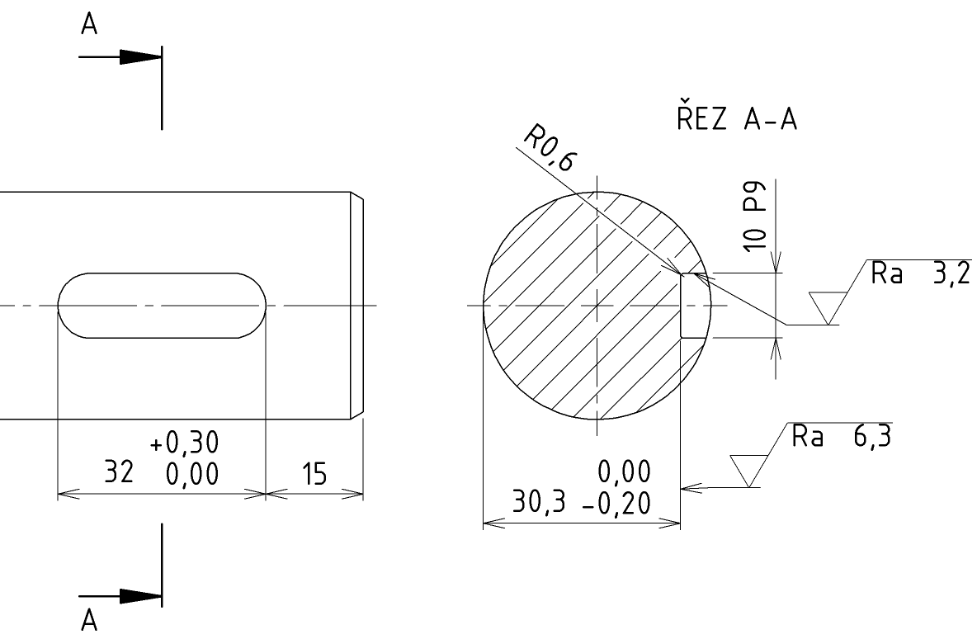
\includegraphics[width=0.65\textwidth]{img/030 img/perodrazka-hridel-screen.png}
    \caption{Popis drážky pro pero na hřídeli}
    \label{fig:keyslot-dwg}
\end{figure}

Vlevo v~nabídce nastavení řezu zvolíme svislou orientaci a řeznou čáru umístíme přibližně do středu drážky.
Zkontrolujeme si, že řez směřuje ven od středu hřídele.
Do zobrazení řezu umístíme středovou značku.

Když máme pohledy nachystané, můžeme začít popisovat.
V~pohledu zakótujeme délku drážky s~podržením klávesy \It{SHIFT} a výběrem obou krajních oblouků.
K~této kótě přidáme oboustrannou toleranci +0,3 a -0.
Dále zakótujeme vzdálenost drážky (krajního oblouku) od čela hřídele, nebo nejbližšího osazení.

Přejdeme do řezu, kde nejdříve zakótujeme šířku drážky.
Této kótě přidáme toleranci \B{P9}.
Dále zakótujeme hodnotu zaoblení dna drážky.
Posledním kótovaným rozměrem je hloubka drážky, kterou zadáme vůči protilehlému oblouku, viz \autoref{fig:keyslot-dwg} vlevo.
Zde přidáme toleranci hloubky, která je pro každou skupinu rozměrů drážek jiná -- zjistíme ji z~tabulky \ref{tab:pera-tesna}.

Posledním krokem je přidání značek drsností povrchu.
U~boků drážky se jedná o~drsnost Ra 3,2 -- značku umístíme na kótu udávající šířku drážky, viz \autoref{fig:keyslot-dwg}  vpravo.
Povrch dna drážky bude mít drsnost Ra 6,3 a umístíme jej na kótu udávající hloubku, opět viz \autoref{fig:keyslot-dwg}  vpravo.

\section{Drážka pro pero v~náboji}
Na výkres si umístíme přední pohled na náš náboj (např. ozubené kolo).
V~kartě \B{Popis} klikneme na \B{Detail}.
Střed detailního pohledu umístíme do středu díry v~náboji a jeho velikost nastavíme tak, aby byla celá drážka viditelná.
Nesmíme zapomenout přidat středové značky.
Vzhledem k~tomu, že díra s~drážkou prochází skrz náboj, její délku kótovat nemusíme.

V~zobrazení detailního pohledu ale potřebujeme zaznačit průměr díry, šířku drážky, její hloubku, velikost zaoblení, drsnosti povrchu a odpovídající tolerance.
Začneme průměrem.
Podržíme klávesu \It{SHIFT} a klikneme nejdříve na první a následně druhou stranu oblouku -- vytvoříme tak průměrovou kótu.
K~ní ještě doplníme toleranci.
Vzhledem k~tomu, že se jedná o~díru, můžeme zvolit například toleranci H7 (možné další viz \autoref{fig:jednotna-dira}).

\begin{figure}[htbp]
    \centering
    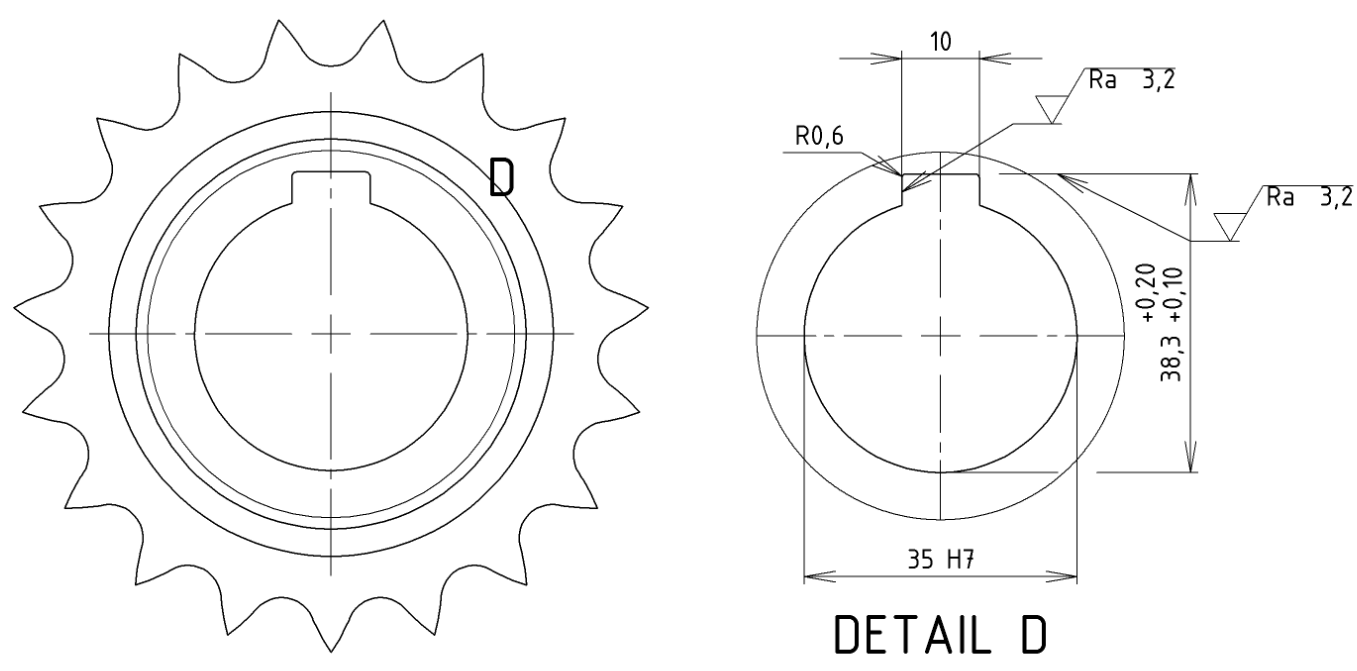
\includegraphics[width=0.6\textwidth]{img/030 img/perodrazka-naboj-screen.png}
    \caption{Plně popsaná drážka na pero v~náboji}
    \label{fig:keyhole-dwg}
\end{figure}

Po průměru musíme zakótovat šířku drážky.
Tato kóta bude mít toleranci P9, jako jsme u~drážek na pero zvyklí.
Hloubku drážky označíme stejně jako u~protikusu na hřídeli -- klikneme na hranu dna drážky, podržíme \It{SHIFT} a klikneme na protilehlý oblouk.
Ještě přidáme toleranci pro danou velikost pera -- zjistíme z~tabulky \ref{tab:pera-tesna}.
Zakótujeme zaoblení a přidáme značky drsnosti povrchu viz \autoref{fig:keyhole-dwg}.

\newpage